\documentclass[xcolor={usenames,dvipsnames,svgnames}, compress]{beamer}

% \usepackage[utf8]{inputenc}
\usepackage{booktabs}
\usepackage{dcolumn}
\usepackage{colortbl}

% \usepackage[style=authoryear-comp, backref=true]{biblatex}
\usepackage{ifxetex}
\usepackage{amsmath}
\usepackage{biblatex}
% 
\usepackage[no-math]{fontspec}

\usetheme{enziteto}

% 
% CLIPS listings
%\usepackage[utf8]{inputenc}
\usepackage{listings}
\usepackage{xcolor}


%
% I asked on stackoverflow for rainbow parentheses
% http://tex.stackexchange.com/questions/235740/rainbow-parentheses-in-lisp-listings
% the palette is from solarized theme
\definecolor{solarized-cyan}{RGB}{42, 161, 152}
\definecolor{solarized-magenta}{RGB}{211, 54, 130}
\definecolor{solarized-yellow}{RGB}{181, 137, 0}
\definecolor{solarized-violet}{RGB}{108, 113, 196}
\definecolor{solarized-red}{RGB}{220, 50, 47}
\definecolor{solarized-orange}{RGB}{203, 75, 22}
\definecolor{solarized-grey}{RGB}{101, 123, 131}

\lstdefinelanguage{clips}
{
  classoffset=0,
  morekeywords ={deffunction, deftemplate, defglobal, defmodule, defrule, deffacts, nil, assert, retract},
  keywordstyle=\bfseries\color{solarized-orange},
  classoffset=1,
  morekeywords ={delcare, salience, run, slot, multislot, clear, reset, facts, exit, agenda, initial-fact, watch, ppdefrule, unwatch, printout, if, then, else, while, loop-count, crlf, read, readline},
  keywordstyle=\bfseries,
  %classoffset=2,
  %keywordsprefix=\?,
  %alsoletter=\?,
  %keywordstyle=\itshape\color{solarized-red},
  classoffset=0,
  sensitive=true,
  morecomment=[l]{;},
  morestring=[b]{"},
  stringstyle=\color{solarized-grey},
  basicstyle=\scriptsize,%\ttfamily\scriptsize,
  numbers=left,
  numbersep=-5pt,
  numberstyle=\tiny,
  showstringspaces=false,
  }

\renewcommand{\ttdefault}{pcr}

% egreg's modulo macro (see http://tex.stackexchange.com/a/34449/21891)
\def\truncdiv#1#2{((#1-(#2-1)/2)/#2)}
\def\moduloop#1#2{(#1-\truncdiv{#1}{#2}*#2)}
\def\modulo#1#2{\number\numexpr\moduloop{#1}{#2}\relax}    

\makeatletter

% a TeX counter to keep track of the nesting level
\newcount\netParensCount@clisp

% Modify how ( and ) get typeset depending on the value of the counter
% (Based on Ulrike Fischer's approach to modifying characters in listings;
% see http://tex.stackexchange.com/a/231927/21891)
\lst@CCPutMacro
\lst@ProcessOther{`(}{{%
    \ifnum\lst@mode=\lst@Pmode\relax%
    \rainbow@clisp{(}%
    \global\advance\netParensCount@clisp by \@ne%
    \else
    (%
    \fi
  }}%
\lst@ProcessOther{`)}{{%
    \ifnum\lst@mode=\lst@Pmode\relax%
    \global\advance\netParensCount@clisp by \m@ne%
    \rainbow@clisp{)}%
    \else
    )%
    \fi
  }}%
\@empty\z@\@empty
% Color its argument based on the value of the \netParensCount@clisp counter
% (modulo 5)
\newcommand\rainbow@clisp[1]{%
  \ifcase\modulo\netParensCount@clisp 5\relax%
  \textcolor{solarized-cyan}{\bfseries#1}%
  \or
  \textcolor{solarized-yellow}{\bfseries#1}%
  \or
  \textcolor{solarized-magenta}{\bfseries#1}%
  \or
  \textcolor{solarized-violet}{\bfseries#1}%
  \else
  \textcolor{solarized-red}{\bfseries#1}%
  \fi
}

% Alternatively, you could simplify the definition of \rainbow@clisp to...
% \newcommand\rainbow@clisp[1]{%
% \textcolor{color\modulo\netParensCount@clisp 5}{#1}%
% }
%   ... but this assumes that the colours have names of the form color<i>,
%   where <i> is a positive integer

%   reset the counter at the beginning of each listing
%   (just in case there were unmatched parentheses in a previous listing)
\lst@AddToHook{PreInit}{%
  \global\netParensCount@clisp 0\relax%
}

\makeatother




\lstnewenvironment{clips-code}[1][]
{\lstset{language=clips,
    #1
  }}
{}






%%% Local Variables:
%%% mode: latex
%%% TeX-master: t
%%% End:


\definecolor{jess-fucsia}{RGB}{170, 0, 127}
\definecolor{violent-green}{RGB}{0, 128, 96}
\definecolor{ny-orange}{RGB}{255, 128, 0}

\hypersetup{
  colorlinks=true,       % false: boxed links; true: colored links
  linkcolor=jess-fucsia,          % color of internal links (change box color with linkbordercolor)
  % citecolor=green,        % color of links to bibliography
  %filecolor=magenta,      % color of file links
  urlcolor=jess-fucsia           % color of external links
}

%%% Local Variables:
%%% mode: latex
%%% TeX-master: t
%%% End:


\lstnewenvironment{java-code}[1][]
{\lstset{language=java,
    #1
  }}
{}


\setbeamertemplate{headline}{}

%%%%%%%%%%%%%%%%%%%%%%%%%%%%%%%%%%%%%%%%%%%%%%%%%%%%%%%%%%%% 
%%%%%%%%%%%%%%%%%%%%%%%%%%%%%%%%%%%%%%%%%%%%%%%%%%%%%%%%%%%% 
%%%%%%%%%%%%%%%%%%%%%%%%%%%%%%%%%%%%%%%%%%%%%%%%%%%%%%%%%%%% 

\begin{document}

\title{CLIPS: Representing uncertainty}
%\subtitle{An Introduction}
\author{Antonio Vergari}
% \institute{Lacam$@$DIB$@$Uniba}
\institute{Università degli Studi di Bari}
\department{Dipartimento di Informatica}
\laboratory{LACAM}
\group{Machine Learning}
\institutelogo{
\includegraphics[width=25pt]{Figures/unibaba}}
\lablogo{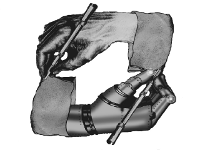
\includegraphics[width=35pt]{Figures/lacam}}

\footnotesize \let\small\footnotesize





{
  \setbeamertemplate{headline}{}
  \setbeamertemplate{footline}{}
  \begin{frame}
    \titlepage
  \end{frame}
}


\begin{frame}
  \frametitle{Uncertainty (like in MYCIN)}
  CLIPS inference engine does not provide any mean to deal with
  uncertain facts or uncertain pattern matching. However, once one is
  able to project rules and matching ont an intermediate
  representation level, uncertainty factors can be introduced at
  different layers.\par\bigskip

  In \textsf{MYCIN}, \textbf{\emph{certainty factors}} (\textbf{CF})
  could be associated to facts in the knowlede base, representing the
  confidence of observing them (positive or
  negative\footnote{Originally they are weights in $\{-1, 1\}$. In the
  following wine example we will consider them normalized in $[0, 100]$}). Observing two
  identical facts with different CFs modifies the WM by introducing
  just one fact with a newly computed CF as follows:
  $$ CF(X, Y) =
  \begin{cases}
    X + Y - XY,& \text{if } X,Y>0\\
    X + Y + XY,& \text{if } X, Y<0\\
    \frac{X+ Y}{1 - \min\{|X|, |Y|\}}. & \text{otherwise}
  \end{cases}
  $$
  

\end{frame}

\begin{frame}
  \frametitle{Uncertainty II}
  Intuitively, seeing more instances of a fact with positive CFs would
  increase the confidence about them, while negative CFs will lower it.\par\bigskip
  Moreover, if we consider patterns $P_1$ and $P_2$ in the LHS of an uncertain rule,
  we can derive the combined CF for the rule in this way:
  $$CF(P_1 \text{ and } P_2) = \min\{CF(P_1), CF(P_2)\}$$
  $$CF(P_1 \text{ or } P_2) = \max\{CF(P_1), CF(P_2)\}$$
  $$CF(\text{not } P) = - CF(P)$$\par
  
  If a rule with an uncertain pattern matches an uncertain fact, the
  resulting CF will be the product of the two CFs (resulting in a
  lower confidence).\par

  If all CF are the max possible values (1), note how we fall into the
  certain pattern matching case.
\end{frame}

\begin{frame}[fragile]
  \frametitle{Wine suggester}
  Back to the wine suggester toy problem, suppose that now the task is
  to suggest the user the name of a wine according to some desiderd
  properties: \emph{color}, \emph{body}, \emph{sweetness}.

  Instead of suggesting only one possible wine, the ES will output a
  list of wines ordered by their CFs.

  \begin{clips-code}
    Do you generally prefer dry, medium, or sweet wines? dry
    Do you generally prefer red or white wines? white
    Do you generally prefer light, medium, or full bodied wines? light
    Is the flavor of the meal delicate, average, or strong? delicate
    Does the meal have a sauce on it? yes
    Is the sauce for the meal spicy, sweet, cream, or tomato? tomato
    Is the main component of the meal meat, fish, or poultry? meat
    WINE                  CERTAINTY
    -------------------------------
    Valpolicella             100%
    Zinfandel                64%
    Cabernet-Sauvignon       40%
    Soave                    40%
    Chablis                  40%

  \end{clips-code}
\end{frame}

\begin{frame}[fragile]
  \frametitle{Extending attributes and rules}
  Derivable facts can still be represented as attribute-value pairs,
  with an added \textsf{certainty} field as a float number (maxed at $100.0$):
  \begin{clips-code}[numbers=none]
    (deftemplate MAIN::attribute
        (slot name)
        (slot value)
        (slot certainty (default 100.0)))
  \end{clips-code}

  We can still use the multislot representation for rules as facts,
  introducing the float property \textsf{certainty} even here to
  express the confidence of the rule
  \begin{clips-code}[numbers=none]
    (deftemplate RULES::rule
        (slot certainty (default 100.0))
        (multislot if)
        (multislot then))
  \end{clips-code}
\end{frame}

\begin{frame}[fragile]
  \frametitle{Wine suggester: example rules}
  Here are some uncertain rules (they start with a certainty of $100$):
  \begin{clips-code}[numbers=none]
    (rule (if has-sauce is yes and  sauce is spicy)
          (then best-body is full))

    (rule (if tastiness is delicate)
          (then best-body is light))

    (rule (if tastiness is average)
          (then best-body is light with certainty 30 and
                best-body is medium with certainty 60 and
                best-body is full with certainty 30))

    (rule (if tastiness is strong)
          (then best-body is medium with certainty 40 and
                best-body is full with certainty 80))

    (rule (if has-sauce is yes and sauce is cream)
          (then best-body is medium with certainty 40 and
                best-body is full with certainty 60))
  \end{clips-code}
\end{frame}

\begin{frame}[fragile]
  \frametitle{Outline strategy}
  \begin{enumerate}[I.]
  \item Ask the users about the wine and meal properties. Assert those
    facts with a $100\%$ certainty
  \item Execute a forward chaining step by using uncertain wine rules to
    assert (possibly) uncertain facts about the derived desired
    properties
  \item Combine uncertain attributes about the same facts according
      to MYCIN rules
  \item Generate the wine list according to the derived attributes
  \item Sort the generated list against the certainty factors
  \end{enumerate}

  In this scenario one may want more identical facts to be asserted in
  the WM:
  \begin{clips-code}[numbers=none]
    (defrule MAIN::start
        (declare (salience 10000))
        =>
        (set-fact-duplication TRUE)
        (focus QUESTIONS CHOOSE-QUALITIES WINES PRINT-RESULTS))
  \end{clips-code}
\end{frame}

\begin{frame}[fragile]
  \frametitle{Questioning I}
  Askable questions are represented as templated facts whose slots
  keep track of valid answers as well as which other questions should
  be asked first (\textsf{precursor}).
  \begin{clips-code}[numbers=none]
    (deftemplate QUESTIONS::question
        (slot attribute (default ?NONE))
        (slot the-question (default ?NONE))
        (multislot valid-answers (default ?NONE))
        (slot already-asked (default FALSE))
        (multislot precursors (default ?DERIVE)))
  \end{clips-code}

  For instance, one cannot ask this second question if the first has
  not already been asked, and its answer was \textsf{poultry}:
  \begin{clips-code}[numbers=none]
    (deffacts WINE-QUESTIONS::question-attributes
        (question (attribute main-component)
                  (the-question "Is the main dish meat, fish, or poultry? ")
                  (valid-answers meat fish poultry unknown))
        (question (attribute has-turkey)
                  (precursors main-component is poultry)
                  (the-question "Does the meal have turkey in it? ")
                  (valid-answers yes no unknown)))
  \end{clips-code}
\end{frame}

\begin{frame}[fragile]
  \frametitle{Questioning II}
  A question can be asked only when its \textsf{precursor} slot is
  empty
  \begin{clips-code}[numbers=none]
    (defrule QUESTIONS::ask-a-question
       ?f <- (question (already-asked FALSE)
                       (precursors)
                       (the-question ?the-question)
                       (attribute ?the-attribute)
                       (valid-answers $?valid-answers))
       =>
       (modify ?f (already-asked TRUE))
       (assert (attribute (name ?the-attribute)
                          (value (ask-question ?the-question ?valid-answers)))))
  \end{clips-code}

  We make it empty by removing matching patterns:
  \begin{clips-code}[numbers=none]
    (defrule QUESTIONS::precursor-is-satisfied
        ?f <- (question (already-asked FALSE) (precursors ?name is ?value $?rest))
        (attribute (name ?name) (value ?value))
        =>
        (if (eq (nth 1 ?rest) and) then (modify ?f (precursors (rest$ ?rest)))
                                   else (modify ?f (precursors ?rest))))
  \end{clips-code}
\end{frame}

\begin{frame}[fragile]
  \frametitle{Uncertain forward chaining I}

  Our modified forward chaining  inference will proceed by selecting
  rules whose LHS matches an asserted attribute. If such an attribute
  exists, then the corresponding pattern is removed from the
  LHS\footnote{Like in the backward chaining setting, we use the WM as
    a blackboard storing only the rules and their parts that we can use again.}\par\bigskip
  \begin{clips-code}[numbers=none]
    (defrule RULES::remove-is-condition-when-satisfied
        ?f <- (rule (certainty ?c1) 
                    (if ?attribute is ?value $?rest))
        (attribute (name ?attribute)
                   (value ?value)  
                   (certainty ?c2))
        =>
        (modify ?f (certainty (min ?c1 ?c2)) (if ?rest)))  
      \end{clips-code}\bigskip
and the global CF of the rule is updated to be the min
of the current CF and the removed pattern CF (since it is the
derivation for the CF of a conjunction of patterns). 
  
\end{frame}

\begin{frame}[fragile]
  \frametitle{Uncertain forward chaining II}

  Again, when a rule fact in our WM gets an empty LHS (\textsf{if}
  multislot), then we can remove it and activate its RHS by asserting
  the corresponding attributes:\par\bigskip
  \begin{clips-code}[numbers=none]
    (defrule RULES::perform-rule-consequent-with-certainty
        ?f <- (rule (certainty ?c1) 
                    (if) 
                    (then ?attribute is ?value with certainty ?c2 $?rest))
        =>
        (modify ?f (then ?rest))
        (assert (attribute (name ?attribute) 
                           (value ?value)
                           (certainty (/ (* ?c1 ?c2) 100)))))
  \end{clips-code}\bigskip

  In this case the CF of the attribute as fact to be asserted is
  equal to the product of the global CF and the RHS pattern
  CF.\par

  Once all rules have been ``fired'', then the WM would contain the
  attributes from the user answers and those derived from
  the forward chaining inference step.
  
\end{frame}

\begin{frame}[fragile]
  \frametitle{Combining uncertain facts}

  Different attribute facts representing the same piece of information are now
  being merged into single facts whose CF is computed as the in MYCIN:\par\bigskip
  \begin{clips-code}[numbers=none]
    (defrule MAIN::combine-certainties
        (declare (salience 100)
        (auto-focus TRUE))
        ?rem1 <- (attribute (name ?rel) (value ?val) (certainty ?per1))
        ?rem2 <- (attribute (name ?rel) (value ?val) (certainty ?per2))
        (test (neq ?rem1 ?rem2)) ;; why is this necessary?
        =>
        (retract ?rem1)
        (modify ?rem2 (certainty (/ (- (* 100 (+ ?per1 ?per2))
                                       (* ?per1 ?per2)) 100))))
  \end{clips-code}
Consider that in this case we are coping with only positive CFs.      
\end{frame}

\begin{frame}[fragile]
  \frametitle{Generating uncertain suggestions I}
  At this point we have to generate the results in terms of
  uncertainty for each wine.\par
  Suppose that we have such a KB about wines, described in terms of
  \textsf{color}, \textsf{body} and \textsf{sweetness}:
  \begin{clips-code}[numbers=none]
    (deffacts WINES::the-wine-list 
        (wine (name Gamay) (color red) (body medium) 
              (sweetness medium sweet))
        (wine (name Chablis) (color white) (body light) (sweetness dry))
        (wine (name Sauvignon-Blanc) (color white) (body medium)
              (sweetness dry))
        (wine (name Valpolicella) (color red) (body light))
        (wine (name Cabernet-Sauvignon) (color red)
              (sweetness dry medium))
        (wine (name Zinfandel) (color red) (sweetness dry medium))
        (wine (name Pinot-Noir) (color red) (body medium)
              (sweetness medium))
        (wine (name Burgundy) (color red) (body full))
        (wine (name Zinfandel) (color red) (sweetness dry medium)))
  \end{clips-code}
\end{frame}

\begin{frame}[fragile]
  \frametitle{Generating uncertain suggestions II}
  Now we can match them against our attributes in the WM:
  \begin{clips-code}[numbers=none]
    (defrule WINES::generate-wines
        (wine (name ?name)
              (color $? ?c $?)
              (body $? ?b $?)
              (sweetness $? ?s $?))
        (attribute (name best-color) (value ?c) (certainty ?certainty-1))
        (attribute (name best-body) (value ?b) (certainty ?certainty-2))
        (attribute (name best-sweetness) (value ?s) (certainty ?certainty-3))
        =>
        (assert (attribute (name wine) (value ?name)
                           (certainty (min ?certainty-1 
                                           ?certainty-2 
                                           ?certainty-3)))))
  \end{clips-code}
  Computing the resulting CFs as min values of the CFs, since we are
  dealing with a conjunction of patterns again.\par\bigskip

  Note that if more attributes facts about a wine are derived, then
  the combine rule will get activated again.
\end{frame}

\begin{frame}[fragile]
  \frametitle{Ordering suggestions}
  The ordering procedure is composed by a rule getting (and
  retracting) the wine fact with highest CF in the WM:
  \begin{clips-code}[numbers=none]
    (defrule PRINT-RESULTS::print-wine 
        ?rem <- (attribute (name wine) (value ?name) (certainty ?per))                
        (not (attribute (name wine) (certainty ?per1&:(> ?per1 ?per))))
        =>
        (retract ?rem)
        (format t " %-24s %2d%%%n" ?name ?per))
  \end{clips-code}

  Wine suggestions getting a CF lower than a certain threshold (let's
  say $20$), can be omitted:
  \begin{clips-code}[numbers=none]
    (defrule PRINT-RESULTS::remove-poor-wine-choices ""
        ?rem <- (attribute (name wine) (certainty ?per&:(< ?per 20)))
        =>
        (retract ?rem))
  \end{clips-code}
\end{frame}

\begin{frame}
  \frametitle{Exercises}

  Add another filter to the output wine list, showing only the top K
  items, where K is a positive integer that shall be asked to the user.
  \par\bigskip
  
  Using this example as a basis, build an exert system for
  recommending some items in a domain you know. For instance, you can
  suggest the user the top movies he could like.\par
  Explicit what are the main attributes for an item to be recommended
  (for the wine domain we had: color, body, sweetness).\par
  Define a hierarchy of intermediate attributes of interest and to get their
  values write the proper questions with the proper \textsf{precursor}
  slot set.\par
  Define a set of uncertain rules to be used for inference.\par\bigskip

  Devise a way to interrupt the question phase when you can already derive
  K suggested items with a threshold > 50.
\end{frame}
\end{document}


%%% Local Variables:
%%% mode: latex
%%% TeX-engine: xetex
%%% TeX-master: t
%%% End:
